This chapter comprises three parts. Section~\ref{sec:background} briefly introduces the background, including the development of artificial intelligence (AI) and robotics, and some related work in automation science. Section~\ref{sec:evolutionary_computation} reviews the development of evolutionary computation,  which is the main technique used in this thesis. It introduces biological evolution, the principles, strengths and weaknesses of evolutionary computation, and its applications. Section~\ref{sec:combine_AI_robotics_animal_behavior} reviews how AI/robotics and animal behavior study benefit from each other. It gives examples of how animal behavior inspires AI/robotics and of how to investigate animal behavior using AI/robotics techniques.  
%As the theme of this thesis is to show how machine intelligence can be used for learning agent behaviors, Section~\ref{sec:animal_behavior_in_nature} presents some examples of animal behaviors observed in nature. Section~\ref{sec:swarm_optimization_swarm_robotics} reviews how animal behavior can be used as inspiration for AI and robotics. Section~\ref{sec:contribution_of_AI/robotics_to_ethology} reviews two methods to study animal behaviors using AI/robotics techniques.  

\section{Background}\label{sec:background}

\subsection{The Development of AI and Robotics}\label{sec:development_of_AI_Robotics}

Intelligence is a natural part of life. Humans and other biological creatures exhibit many behaviors (e.g., decision making and foraging) that require intelligence. However, intelligence is not a property that is limited to biological creatures. It should be equally applicable to machines. The term AI emerged in a conference in 1956 at Dartmouth College, where several researchers (e.g., Marvin Minsky and John McCarthy) who were later considered pioneers of this field, discussed the development of digital computers and the future of AI. The definition of AI is still a disputed topic.  Some researchers argue that AI is to simulate the intelligent behaviors that are observed in humans and other biological creatures using computers or machines. That is, an intelligent machine should be able to exhibit behaviors similar to that of living creatures when encountering the same problems~\cite{Schildt1985}. Others give the following definition: ``Artificial Intelligence is the study of mental faculties through the use of computational models''~\cite{Charniak1985}. According to Fogel~\cite{Fogel1995}, an intelligent system should know how to make decisions in order to fulfill a goal (e.g., solving a problem). In other words, instead of pre-programming the machine using human's knowledge, it should be able to learn and adapt. In~\cite{Minsky_1991}, Minsky argued, ``Why can't we build, once and for all, machines that grow and improve themselves by learning from experience? Why can't we simply explain what we want, and then let our machines do experiments or read some books or go to school, the sorts of things that people do?'' In 1950, Turing~\cite{Turing_1950} proposed an imitation game which is nowadays known as \textit{Turing test} to discuss a question: ``Can machine think?''. Although whether a machine could pass the \textit{Turing test} or not was beyond the consideration at that time, it was accepted as a notion that a machine could learn and adapt to mimic human behavior. %Many promising achievements have been made to enable machines to exhibit a variety of intelligent behaviors since then. 

%One of the most representative examples is IBM's chess program (Deep Blue). It defeated the champion of the world chess (Gary Kasparov) in 1997~\cite{Newborn1992}, which provides evidence that a computer program can even outperform a human expert in terms of decision-making ability. 
In the 1970s, the emergence of expert systems---computer programs that mimic human experts' decision-making capability~\cite{Jackson1998}, significantly promoted the development of AI. An expert system can solve complicated problems through reasoning about the knowledge (which is mainly represented as \textit{if-then} rules) it has. In an expert system, there are two elements---knowledge base and inference engine. Knowledge base includes facts and rules that are known to the system. Inference engine utilizes the facts and rules to make decisions and derive new rules, which are then stored in the system to update the knowledge base. Expert systems have many real-world applications such as medical diagnosis \cite{Jonathan1990}, scientific hypothesis formation \cite{Robert1993}, and structural safety monitoring \cite{Salvaneschi1996}. 

The rules in an expect system can be expressed using Boolean logic or Fuzzy logic. In Boolean logic, every condition in the rules is either true or false. Fuzzy logic was introduced by Zadeh~\cite{Zadeh:IC:1965} to describe a degree of truth. For example, a cup with water is described as ``full (1)'' or ``empty (0)'' using Boolean logic; however, in Fuzzy logic, it can also be described using some fuzzy expressions such as ``almost full'', ``half full'', ``near empty''. Fuzzy logic is commonly used in our daily life. An example rule in an expert system using Fuzzy logic is: \textit{IF the temperature is cold, THEN turn the heater on.} In stock markets an old saying is: ``buy low, sell high''. However, whether the stock value can be considered as low or high depends on the stock curves in a particular situation. Fuzzy systems have many commercial applications, such as in air conditioners, digital cameras and hand writing recognition. 

Another representation of AI is the neural network, which mimics the processing ability of nervous systems of biological organisms (especially human brain). Through a combination of weights and excitation functions (e.g., sigmoid function), neural networks can accomplish many tasks observed in humans, such as pattern recognition and image processing. 

%Over decades, researchers are dedicated to making machine exhibit behaviors using symbolic representations to mimic human behaviors. The rules executed in a machine are usually programmed. However, when we consider the natural evolutionary process, it takes ages for humans to pick up a particular intelligence behavior. It is straightforward to say that through simulating the natural evolutionary process, a machine could exhibit intelligence that may be unpredictable by the programmers~\cite{Fogel1995}. In other words, intelligence can be evolved, and this is the main topic discussed in the rest of this thesis. 
%In 1959, a program was written to play checkers~\cite{Samuel1959}. 

%In the early stage of AI, the program is only run on a computer, and the input is digital. With the development of AI and hardware, researchers start to combine AI with moving machines such as a robot. Different from the digital world in a computer, the environment that a robot operates on is much more complex. The input of the system can be digital, analog or hybrid, which makes the modeling/abstract of the operating environment challenging. 
%Robotics is a field about making machines that can move in several ways to accomplish certain tasks.

Robotics is a field in which machines interact with their environment to accomplish certain tasks. While AI and robotics are not essentially connected, they are often used together to make robots appear intelligent. For example, a robot with AI can move autonomously and make decisions while interacting with the environment it is operating in. Through combining AI and robotics, machines can be created in such a way that they can learn and adapt to a changing environment. In \cite{Cully2015}, a robot was built to be capable of automatically finding compensatory behaviors after going through damage in a locomotion task. 
%Instead of only executing repetitive tasks such as the robotic manipulators in a car assembling line,

There are two common paradigms adapted for the control of a robot: deliberative paradigm and reactive paradigm. In deliberative paradigm, the robot operates on a top-down fashion and its action mainly depends on planning. A typical cycle is: $sense \rightarrow plan \rightarrow act$. In the sensing stage, the robot gets the information from the world based on sensors such as cameras, infrared sensors, etc. After pre-processing, this information would be passed to the central control architecture which integrates all the sensing information and reasons about it. Based on the knowledge the robot has, it can decide which action to take to fulfill a goal (e.g., to maximize its reward). This paradigm has led to many successful applications. The pioneer work is~\textit{Shakey the robot} which is capable of reasoning about its own actions~\cite{Nilsson1984}. In this work, the robot is operating under simplified conditions (e.g., uniform color and flat floor). Further work has been done since then to enable robots to tackle complex and changing environments \cite{Dimitrov:ICSMC:2013}. In the reactive paradigm, the robot makes decisions based on $sense \rightarrow act$ without deliberate reasoning or planing. Instead of building a central reasoning system to integrate all the sensory information, the robot could process it in parallel. Some famous robots using the reactive paradigm are Allen \cite{Brooks1986}, Herbert \cite{Buchanan:1984} and Genghis \cite{Brooks:1989}. 
%To accomplish a complex task, researchers may need to combine different architectures integrated in a cognitive manner. This lead to a new research area---cognitive robotics. It is argued that intelligence emerges from interaction of different layers of $sensor \rightarrow act$ pairs. Another paradigm adapted widely nowadays is subsumption architecture~\cite{Brooks1986}
%This could enhance the robustness of the robotic control system. 
 
\subsection{Introduction of Automation Science}

With the development of AI and robotics, intelligent and automation systems were commonly used to assist scientific research. Since the first clinical automated laboratory management system \cite{Steinlechner2001} was created in 1993, such systems are increasingly used in drug discovery, agriculture, energy labs, etc. In order to accelerate the experimental process, researchers take advantage of intelligent and automation systems to help, for example, collect and analyze data, as this can be time-consuming and tedious if carried out manually. The ideal situation is to make a machine conduct scientific research automatically without or with little human intervention. It could then conduct experiments day and night in a constant manner without any tiredness.
%The question of whether it is possible to automatically conduct scientific research is very interesting in theory, and it also involves a lot of practical work which needs to be solved. It is desirable that machines can automate the whole process of scientific research. 
          
The field of automation science has been developed to a great extent because of the increasing demands of drug industry and relevant fields of biology and chemistry. High-throughput screening (HTS) systems~\cite{Persidis_1998} are one of the early efforts. HTS systems can, for instance,  prepare, observe and analyze data automatically, thus greatly enhancing the speed of experimental process. Recently, King, et al.~\cite{King_2004, King_2009} have built a ``Robot Scientist''---Adam.  It can automatically generate functional genomics hypotheses about the yeast~\textit{Saccharomyces cerevisiae} and carry out experiments to test and refine the hypotheses based on techniques developed in AI and robotics. Adam could automatically conduct the cycles of scientific experiments: forming hypothesis, initializing the experiments, explaining the results and verifying the hypothesis, and then repeating the cycle. The functional genomics hypotheses are autonomously generated by intelligent software and the experiments are conducted through coordinating different components in the automated system~\cite{King_2004}. This ``Robot Scientist'' \cite{King_2009} is able to conduct plenty of experiments and observations a day. In~\cite{Gauld_2000}, Gauld et al. have developed a digital automated identification system (DAISY) to identify biological species automatically with high accuracy using an advanced image processing technique. This technology has gone though great improvement in recent years, enhancing the possibility of automation, or at least semi-automation, in the process of routine taxonomic identification. In~\cite{MacLeod_2010}, MacLeod et al. reported that an imaging system that is originally designed for identifying marine zooplankton was used by the US government for automatically monitoring Deepwater Horizon oil spill. They argue that taxonomists and researchers in machine learning, pattern recognition as well as AI should collaborate with each other in order to better identify and name biological species. 

Drawing on approaches from various research areas especially AI and robotics, intelligent and automation systems are playing a vital role in scientific research, allowing researchers to conduct experiments more efficiently. It is argued that the revolution of automation science may emerge in a few decades~\cite{King_2009}.
%%Therefore, Adam is the integration of robotic system, automatic control technology as well as artificial intelligent. , which makes it possible to go through the whole process of experiments

\section{Evolutionary Computation}\label{sec:evolutionary_computation}

Evolutionary computation is a field studying techniques that are inspired by biological evolution. We use an evolutionary computation technique to automate the generation of models during the system identification process. 

This section is organized as follows. Section~\ref{sec:natural_evolution} introduces biological evolution. Section~\ref{sec:intro_evolutionary_computation} details the principles, strengths and weaknesses of evolutionary computation. Section~\ref{sec:application_evolutionary_computation} presents three main applications of evolutionary computation and related work.
%It is a stochastic search method and uses trial-and-error to guide the search process.

\subsection{Biological Evolution}\label{sec:natural_evolution}

Biological evolution is about how living organisms evolve to adapt to environmental changes. According to Darwin's Theory of Evolution~\cite{Darwin_1859}, individuals compete for survival. The individuals that are better adapted to the environment tend to reproduce more. This phenomenon is regarded as~\textit{natural selection}. From another point of view, the genes that help the species survive better would have a higher chance of be preserved and passed on to the next generation, while the genes that are harmful would be abandoned. 
%There are heritage (e.g., through sexual reproduction) and random mutation among species' genes. 

%Their offspring are more likely to inherit such advantageous function and this function would be passed to the next generation. The other members without the advantageous function are less likely to reproduce. 
Natural selection tends to accumulate beneficial genetic mutations \cite{Desai2007}. Suppose that some members in a species have evolved a functional organism that is very useful (e.g., a wing that can fly). This makes these members easier to find food or avoid predators. The offsprings that inherited such advantageous function are more likely to live longer and reproduce more; the other members without the advantageous function are less likely to reproduce. Natural selection helps the species to adapt better to their environment. At the same time, it also accelerates the extinction of the species that can not adapt well to environmental changes. For instance, the dinosaur used to be a dominant species in the past. Their size was a big advantage when the climate was mild. However, as the climate changed dramatically (e.g., extremely cold or hot), the big body was no longer an advantage as it needed too much energy. This may accelerate the extinction of dinosaurs \cite{Russell1965}. 

Coevolution is a special form of evolution, which involves the simultaneous evolution of two or more dependent species. A typical example of coevolution is fox and rabbit or parasite and host. In nature, survival abilities of species are coupled. That means, the survival ability of one particular species depends not only on its DNA (genes) grouped as chromosomes, but also on other species. For a specific species, there can be three relationships with other species: beneficial, harmful and neutral \cite{BiLi2009}. Therefore, through permutation and combination, the relationship between two species can be summarized in Table~\ref{tab:relationship_species_coevolution}. It includes six concrete relationship: reciprocity, neutral, symbiosis, amensalism, predation and antibiosis \cite{BiLi2009}.

\begin{table}[!t]          
  \centering                     
  \caption{The relationship between different species that coevolve. Symbols `+', `-' and `0' represent beneficial, harmful and neutral in a relationship, respectively. For example, ``+, -'' indicates A benefits and B get harmed.}
  \label{tab:relationship_species_coevolution} 
  \renewcommand{\arraystretch}{1.7}
  \begin{tabularx}{430pt}{l|l|l|l}                                                    
    \hline                                                                %\hline: the herizon line
     & \multicolumn{3}{c}{the influence of species A } \\                       % use & to divide the columns         
    \hline
    & +,+ (reciprocity)  & +,0 (symbiosis)   & +,- (predation)   \\
    the influence of species B & 0,+ (symbiosis) & 0,0 (neutral) & 0,- (amensalism)  \\
    & -,+ (predation)    & -,0 (amensalism) & -,-(antibiosis) \\
    \hline
  \end{tabularx}
\end{table}

\subsection{Introduction of Evolutionary Computation}\label{sec:intro_evolutionary_computation}

\subsubsection{Principles}\label{sec:principles_evolutionary_computation}

Based on the principle of biological evolution, the genetic algorithm (GA) was proposed by Holland in 1960s \cite{Halland_1992}. There is a population of solutions in the GA. The solution for a given problem is represented as a chromosome, which contains several genes. Each gene could be a bit, integer, or floating-point number. The GA is driven by a fitness function, which defines the quality of the candidate solutions in the population. The evolutionary process is to optimize (e.g., maximize) the fitness of the individuals. There are three genetic operators: selection, crossover and mutation.  In each generation, the individuals with high fitness have a higher chance of being selected to the next generation and producing offsprings (e.g., through crossover). Mutation can be, for example, realized by randomly changing a particular gene. Mutation in GA serves the same function as it is in biological evolution. It creates diversity in the population. 
%For example, some gene in the chromosome may be randomly replaced by another gene. 

There are other types of evolutionary algorithms. Fogel, Owens and Walsh invented evolutionary programming (EP)~\cite{Fogel1966}. Rechenberg and Schwefel introduced evolution strategies (ES)~\cite{Rechenberg1994, Schwefel1995}, which are mainly dealing with real-value continuous optimization problems. In the early 1990s, another type of evolutionary algorithm called genetic programming (GP) was presented by Koza~\cite{Koza1992}. Fig.~\ref{fig:evolutionary_algorithm_classification} shows a brief classification of evolutionary algorithms. 

\begin{figure}[htbp]
  \centering
  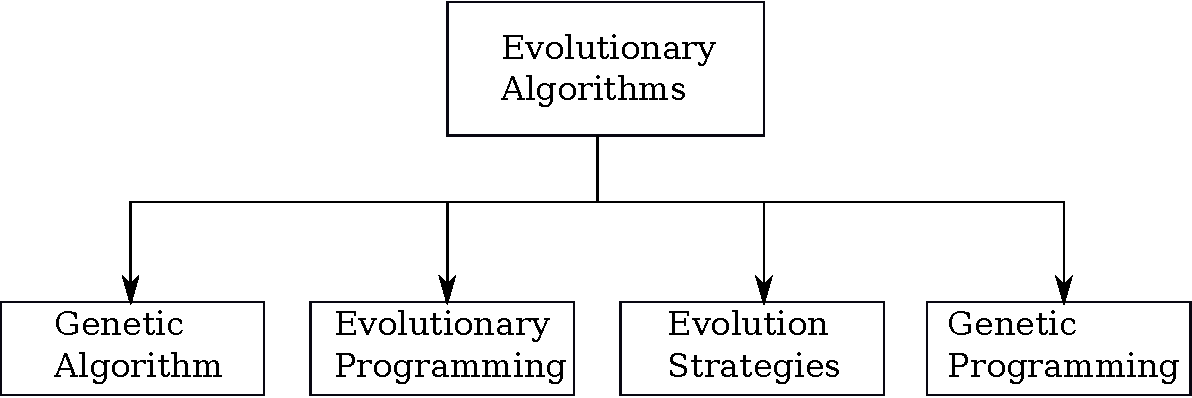
\includegraphics[width=4.2in]{evolutionary_algorithm_classification.pdf}
  \caption{Classification of evolutionary algorithms}
  \label{fig:evolutionary_algorithm_classification}
\end{figure}

The implementation of evolutionary algorithms follows a general flow during the operation process. They can be divided into five steps: initialization, evaluation, mutation, selection and termination. At the beginning, a random population of individuals is initialized. Each individual is represented as a string (chromosome), which contains several genes (e.g., floating point numbers). These strings encode the candidate solutions. Different chromosomes are then evaluated using a predefined fitness function. The fitness of individuals in the population only depends on their own chromosomes. Selection happens after evaluation of each individual, and the ones with higher fitness are more likely to be selected to the next generation and have offsprings. The offsprings would go through mutation, which helps to maintain the diversity of the whole population.  Fig.~\ref{fig:evolutionary_algorithms_flow} show a diagram of how the evolutionary algorithms proceed. 

%That means in different generations, the fitness of individuals who own the identical chromosome is constant.
\begin{figure}[htbp]
  \centering
  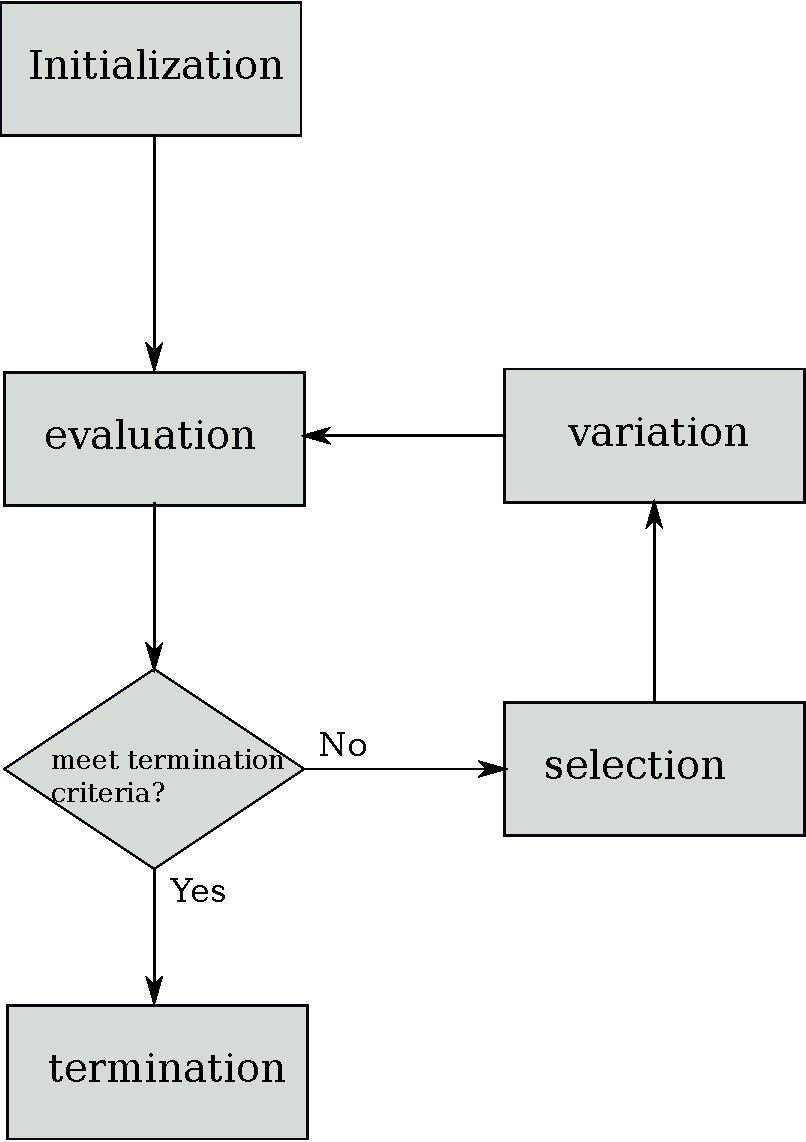
\includegraphics[width=2.5in]{evolutionary_algorithms_flow.pdf}
  \caption{This diagram shows the flow of evolutionary algorithms. Adapted from \cite{Eiben:Nature:2015}}
  \label{fig:evolutionary_algorithms_flow}
\end{figure}

As mentioned before, the species in nature are not independent, and they coevolve. The different kinds of relationship in Table~\ref{tab:relationship_species_coevolution} show that the evolution of individuals among species are coupled. Coevolutionary algorithms, which coevolve simultaneously two or more populations, are widely adapted to solve real-world problems \cite{Rosin_1997, Bongard2005, Zhou2006, tan2006coevolutionary}. In principle, coevolutionary algorithms can be considered of comprising several sub-algorithms, each of which could be an evolutionary algorithm. These sub-algorithms interact with each other in the fitness calculation process. In other words, the fitness of individuals in one population not only depends on its own chromosome, but also on the performance of other individuals from another population during the coevolutionary process. 

%Figure \ref{Fig: diagram_coevolution} shows a schematic diagram of a coevolutionary algorithm with two populations.
%\begin{figure}[htbp]
%  \centering
%  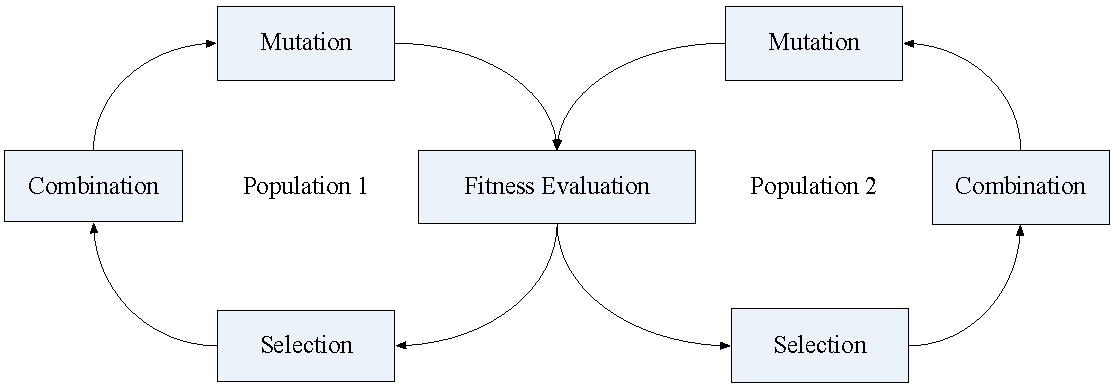
\includegraphics[width=4.2in]{diagram_co_evolution.pdf}
%  \caption{A schematic diagram of a coevolutionary algorithm with two populations.}
%  \label{Fig: diagram_coevolution}
%\end{figure}

The essential difference between evolutionary algorithms and coevolutionary algorithms is the way of fitness evaluation. In coevolutionary algorithms, the individual's fitness depends on its performance and that of the individuals from the other populations. Coevolutionary algorithms are generally divided into two categories---competitive coevolutionary algorithm (Comp-CEA) and cooperative coevolutionary algorithm (Coop-CEA). A Comp-CEA assesses each individual by its competitive performance with respect to its opponents, while Coop-CEA assesses each individual by its cooperative performance with respect to its co-operators. As discussed by Dawkins and Krebs \cite{Dawkins_1979}, competitive coevolution can produce the phenomena of ``arm races'' where complexity of each population increases. The evolution of one population may drive another population to evolve new strategies, which makes the individuals of both populations evolve a higher level of complex behavior. Generally, Coop-CEA is applied to the situation in which the problem can be divided into several sub-problems. Several cooperative populations are evolving simultaneously, and each individual of a sub-population represents a part of the solution. The fitness of an individual could be the quality of the solution formed by the combination of the individual with those from other sub-populations. In the rest of the thesis, we only discuss Comp-CEAs, which will also be referred to as coevolutionary algorithms in general.
%Evolutionary algorithms evaluate individuals by their chromosomes, which are independent of those in other individuals in the population. Coevolutionary algorithms evaluate individuals based on their relative performance compared with the individuals from the other populations.

In coevolutionary algorithms, the fitness of individuals is called subjective fitness \cite{John_2004}. An individual's subjective fitness is based on the performance of its temporary opponents from the current generation or a combination of current and past generations. The fitness of individuals with the same chromosome may vary in different generations because of changing opponents. Conversely, the fitness in evolutionary algorithms is called absolute or objective fitness.

%Comp-CEA can be applied in a single population or in multiple populations. The single-population Comp-CEA is realized by competition between individuals within the same population. 
Suppose there are two populations in a coevolutionary algorithm. One is called ``learner'', and the other is called ``evaluator''. Let $L$ represent a set of learners and $E$ represent a set of evaluators. For a learner, a simple way of calculating its subjective fitness is to count the number of evaluators (in the current population) that this learner defeated~\cite{Angeline_1993}. It is described in equation~\eqref{equ:simple_fitness_calculation} as follows (reproduced from \cite{BiLi2009}):

\begin{equation}\label{equ:simple_fitness_calculation}
\forall i \in L \Rightarrow C{F_i} = \sum\limits_{j \in E,{\kern 1pt} i{\kern 1pt} \text{defeats} {\kern 1pt} j} 1.
\end{equation}

$C{F_i}$ is the fitness of learner \textit{i}. 

Another fitness calculation approach is called competitive fitness sharing \cite{Rosin_1997} as described in the following (reproduced from \cite{BiLi2009}):

\begin{equation}
\forall j \in E \Rightarrow {N_j} = \sum\limits_{k \in L,{\kern 1pt} k{\kern 1pt} \text{defeats} {\kern 1pt} j} 1.
\end{equation}

\begin{equation}\label{equ:competitive_fitness_sharing}
\forall i \in L \Rightarrow C{F_i} = \sum\limits_{j \in E,{\kern 1pt} i{\kern 1pt} \text{defeats} {\kern 1pt} j} {\frac{1}{{{N_j}}}}.
\end{equation}

${N_j}$ represents the number of learners that could defeat evaluator \textit{j}.  

In competitive fitness sharing~\cite{Rosin_1997}, the learner that could defeat the more competitive evaluator gets higher reward. For example, if learner $i$, in a population is the only individual to defeat evaluator $j$, this learner's accumulative fitness is added by $1$, as $N_j$ is equal to $1$ in Equation~\eqref{equ:competitive_fitness_sharing}. The aim of using competitive fitness sharing is to preserve/award the learner that possesses genetic material that is worth passing to the next generation. 

There are many ways to choose the evaluators (temporary opponents). Random Pairing \cite{Panait_2002} means finding a random temporary opponent for each learner. In single elimination tournament \cite{Tan_2007}, all the individuals randomly match, and the losers are taken out and winners are selected into next the round of random match. Alternatively, Round Robin \cite{Panait_2002} pairs all evaluators temporarily with each learner. There are also other ways such as K-random opponent \cite{Tan_2007} and shared fitness \cite{Rosin_1997}. The evaluation time for random pairing is the shortest, but the performance is the worst; the calculation time for round robin is the longest, but the performance is the best \cite{BiLi2009}. In the coevolutionary method (\textit{Turing Learning}) proposed in this dissertation, a fitness calculation similar to Round Robin is chosen.
%The general Comp-CEA involves two or more species, and it simulates the predator and prey relationship in the ecological coevolution. Different species rotate as learner and evaluator during the coevolution process.
%In fitness sampling, the selected temporary opponents should have a high fitness value in the last generation. 

\subsubsection{Strengths}

The advantages of evolutionary computation can be summarized in the following \cite{Fogel:1997}:

\begin{itemize}
\item \textit{Conceptually Simple:} Evolutionary computation techniques can be implemented using simple genetic operators (e.g., selection, crossover, mutation) as mentioned in Section \ref{sec:principles_evolutionary_computation}. 

\item \textit{Task-independent:} Evolutionary computation techniques can be used for optimization. Many tasks in reality can be treated as function optimization or black-box optimization problems (which will be detailed in Section \ref{sec:black_box_optimization}). 

\item \textit{Parallel Computing:} Evolutionary algorithms can run in parallel to accelerate the evolutionary process. The individual can be evaluated independently according to the fitness function. However, the selection and recombination process is normally done in series.

\item \textit{Robust to Changes:} Evolutionary computation is robust to changes of circumstances. Once the circumstances have changed, the evolved solutions can be used as a start for further development without the need to restart the whole process \cite{Hornby2011}.
 
\end{itemize}

Apart from the general advantages of evolutionary computation, coevolutionary algorithms have the following two advantages:

\begin{itemize}
\item \textit{Open-Ended Evolution:} Coevolutionary algorithms can create an open-ended evolution for each population due to the complex interaction between the competing populations during the coevolutionary process. Such open-ended evolution could encourage the appearance of new building blocks, thus maintaining the diversity of populations. In Darwin's natural selection, this phenomenon is referred to as ``arm race''~\cite{Dawkins_1979}, which leads each species to continuously improve.  

\item \textit{No Absolute Fitness Needed:} Coevolutionary algorithms can be applied to solve problems in which absolute fitness can not be effectively defined. For example, when evolving a chess program, it is challenging to define a fitness to qualify it, although playing against fixed programs would be an option \cite{gross2002evolving}. An alternative way of evaluating a chess program is making it play with competing programs and then calculating its subjective fitness~\cite{Angeline_1993, David2014}. 
\end{itemize}

\subsubsection{Weaknesses}

The main weakness of evolutionary computation is that it usually requires significant (computational) efforts to obtain good solutions. In simulation, this would not necessarily be a problem; however, if the evaluation needs to be conducted on a physical system, it would take a long time and may also be expensive.

There is no guarantee that using evolutionary computation techniques can always find the optimal or right solution. This may limit its use on some tasks that have a high demand of safety, as an occasional error may cause a system failure.

Apart from the general disadvantages of evolutionary computation techniques, in particular, there are three main pathologies of coevolutionary algorithms:

\begin{itemize}

\item \textit{Red Queen Effect:} When the Red Queen effect happens, two populations compete with each other and their subjective fitness keeps increasing during the coevolutionary process, however their objective fitness does not constantly improve. On the other hand, their objective fitness increases, but the subjective fitness does not reflect such situation \cite{Bongard2005}. 
%For a particular population, when~\textit{Red Queen Effect} happens, the tendency of subjective fitness and objective fitness curves (over generations) may be opposite \cite{kauffman1995}. For example, the increase of an individual's subjective fitness may correspond to the decrease of its objective fitness. 

\item \textit{Cycling:} In coevolutionary algorithms, the criteria (temporary opponents) used for evaluating an individual (solution) is changing over generations. As a consequence of this, some solutions in the previous generations may be lost and rediscovered later. This phenomenon is referred to as \textit{cycling} \cite{John_2004}. A method of overcoming the problem of ``cycling'' is ``hall of fame''\cite{Rosin_1997}. ``Hall of fame'' remains the good individuals from the previous generations, and these obtained individuals may be selected to be temporary components to evaluate the individuals from the competing population in the current generation.

\item \textit{Disengagement:} During the coevolutionary process, when one population is entirely better than the other, disengagement will occur. In this case, the selection criteria will not make sense, since the subjective fitness of individuals in each population is constant. The lack of selective pressure would cause each population to diverge. Common methods for addressing the disengagement problem is ``resource sharing'' \cite{Juille98coevolvingthe} and ``reducing virulence'' \cite{John_2004}. 

%The diversity of populations will converge into zero, and it is impossible to form ``arm race''~\cite{Dawkins_1979}. 
%disengagement can be avoided by selecting for individuals that exhibit reduced levels of “virulence”, rather than maximum ability to defeat coevolutionary adversaries.

\end{itemize}

\subsection{Applications of Evolutionary Computation}\label{sec:application_evolutionary_computation}

Evolutionary computation techniques are widely used for solving various engineering tasks such as image processing, pattern recognition, robot control and system identification. 
Many real-world applications of evolutionary computation can be found. In the area of nanophotonic light trapping, a need is the development of low cost thin film solar photovoltaic technologies. A traditional way is fixing the structure according to an expert's experience and trying to find good parameters. In~\cite{Wang2013}, a highly efficient light-trapping structure was designed using genetic algorithm. It was shown that this structure can increase the trapping efficiency three times compared with the classic design. Another successful example is using evolutionary algorithms to design antennas for NASA's Space Technology spacecraft~\cite{Hornby2011}, and one of the antennas was used in the mission. The antenna is a critical device for a spacecraft to communicate with the ground, as faulty communication may cause data loss or even the crash of the spacecraft. The antennas designed using evolutionary algorithms are significantly better than those designed by human experts. 
%The high efficiency achieved by the new design is far beyond the reach of traditional design. 

In the following sections, we will focus on three main fields in which evolutionary computation plays a role.

%For example, in a traveling salesman problem, in which the task is to find the best combination of route of cities (input) that can minimize the length of tour of visiting all cities. 

%Such algorithm has been successfully applied in intelligent games, for example, Tic-Tac-Toe \cite{Angeline_1993} and function optimization \cite{Tan_2007}. The multi-species Comp-CEA has been successfully applied in intelligent games such as Tic-Tac-Toe \cite{Rosin_1997}, function optimization, multi-objective optimization \cite{Tan_2007}, pattern recognition, the design of nonlinear controllers and artificial neural networks \cite{Floreano_1997}.

\subsubsection{Black Box Optimization}\label{sec:black_box_optimization}

\begin{figure}[!t]
  \centering
  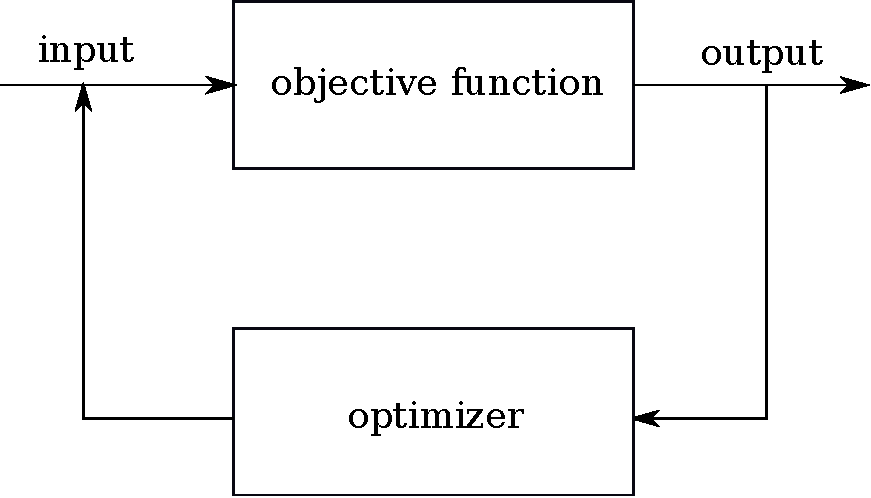
\includegraphics[width=3.2in]{black_box_optimization.pdf}
  \caption{This diagram shows the process of black box optimization. The task is to find a candidate solution (input) that can optimize (e.g., maximize or minimize) the objective function.}
  \label{fig:black_box_optimization}
\end{figure}

A prominent application of evolutionary computation is black box optimization. Black box optimization refers to optimizing an objective function without assuming the hidden structure (e.g., linear or differentiable) \cite{BBOC2015}. In particular, the aim is to find a set of inputs that can maximize or minimize the output of the objective function. Fig.~\ref{fig:black_box_optimization} shows a diagram of the black box optimization. In the following, we list a few cases that evolutionary computation could be applied to solve hard optimization problems \cite{Melvin:PhD:2014}. 
%Evolutionary algorithms,  unlike many traditional search algorithms such as the greedy local search algorithm~\cite{Gutin200281}.
%Another advantage of using evolutionary algorithms for designing is once the fitness function was changed, it can quickly come up with another design can fit the purpose. 

\begin{itemize}

\item \textit{High-dimensional:} As the dimension, $n$, of the objective function increases, the search space increases exponentially. This is called ``curve of dimension'' by Bellman~\cite{Bellman1957}. If we have to optimize a function that has $30$ dimensions, and each dimension only has $20$ parameter values to be selected, for a grid search in which all the possible solutions are evaluated, it will take $20^{30}$ evaluations. Suppose that each evaluation takes $1\mu s$, the grid search would take more than $3\cdot 10^{31}$ years. Using evolutionary computation techniques can shorten the time to find a good solution. 

\item \textit{Multi-Model:} Multi-model means a system (function) has more than one optima (e.g., Rastrigin Function). The one(s) with the best fitness value is (are) considered as global optima, and the other are considered as local optima. These local optima can be misleading for gradient-based search algorithms (e.g., \textit{hill climbing} algorithm), as the solutions may get trapped. Evolutionary algorithms are shown to be effective to find global optima \cite{Hansen2003}. %For example, in the optimization of a multi-layer forward neural network, there may be multiple representations that could produce the same output because of the symmetrical structure of the hidden neurons.

\item \textit{Non-separable and non-differential:} A function, $g(x_1, x_2, \cdots, x_n)$ is non-separable, if it can not be expressed as: $g(x_1, x_2, \cdots, x_n) = g(x_1)g(x_2) \cdots g(x_n)$. For a separable function, it would be much easier to optimize each variable separately. However, for non-separable system, the variables can be coupled. Also, the function may not be differentiable, which makes many mathematical optimization algorithms (e.g., quasi-Newton BFGS algorithm~\cite{Dennis1977} or conjugate gradient algorithm~\cite{Shewchuk1994}) infeasible. %The state-of-the-art of the evolutionary algorithm for black box optimization in contentious domain is Covariance Matrix Adaptation Evolution Strategy (CMAES)\cite{Hansen2003}.

\item \textit{Multi-objective:} When encountering real-world problems, we usually need to deal with multiple objectives, which need to be optimized simultaneously. For example, when designing a car, the engineers need to consider the shape, performance of the engines and cost. As some of the objectives are conflicting, the designer should find a Pareto optimal solution~\cite{Fonseca1995}, in which none of the values of the objective functions can be increased without decreasing the value of other objective functions. Evolutionary multi-objective optimization is a technique to generate Pareto optimal solutions. For a review, see~\cite{Fonseca1995}. 

\end{itemize}

\subsubsection{Evolutionary Robotics}\label{sec:evolutionary_robotics}

Another application of evolutionary computation is evolutionary robotics, in which the controller and/or morphology of a robot are automatically generated \cite{Doncieux2015, Eiben:2015:ER}. The user considers the robot as a whole and only needs to specify the optimization criteria which are represented by a fitness function. The fitness function could be single-objective or multi-objective. The aim is to optimize the fitness using evolutionary algorithms. 

To optimize controllers of a robot, the normal procedure is as follows. First, an initial population of random controllers is generated. Each controller is represented by a chromosome. If the controller is a neural network, the chromosome could be a vector of real numbers. Each controller is tested on the robot (in simulation or reality), and the robot's performance for some specific task is measured and evaluated using a pre-defined fitness function. The `fitter' controller (i.e., with higher performance) has a higher chance of being selected and generating offspring in the next generation. This process iterates until a good solution is found. 

%Another potential method of designing robot controllers is behavior-based approach, where the designer divides the whole system into several simple parts intuitively. These separate parts are then integrated all in once through a coordination mechanism---competitive or cooperative coordination~\cite{Brooks1986}. In competitive coordination, only one part has an effect on the output of the robot, while in cooperative coordination, several parts contribute to the output of the robot with different weights. The behavior-based method was shown to be very robust in many tasks such as gait control in locomotion and object transport. The challenge of designing robot controller and/or morphology using behavior-based method is it requires a lot of experience from the designer. Moreover, when the system is highly coupled, separating the whole design into different parts may not be a good strategy. However, evolutionary robotics provides the designer an alternative way of controlling the robot as a whole, rather than focuses on the details of each separate component. The synthesized control system is a result of self-organized process. %A schematic diagram showing the design process of evolutionary method and behavior-based method is shown in Fig.~\ref{}.

A common control structure adapted in evolutionary robotics is the artificial neural network due to its simple representation \cite{Floreano_1997, Floreano2008:NN}. According to the types of control strategies, different neural networks can be chosen (forward neural networks and recurrent neural networks, etc.). After selecting the structure of the robot controller, evolutionary algorithms are used for optimizing the weights of the neural networks. Note that one can even evolve the structure (topology) and weights of the neural networks~\cite{Kenneth2002}. 
%Tree-based structures like LISP are widely used in evolutionary programming~\cite{Koza:1992}.  The \textit{building blocks} method was proposed by Brooks~\cite{Brooks92artificiallife}. However, these blocks are described using high-level languages, which are not suitable for evolution in the low level. 

There are two main research aims in evolutionary robotics \cite{Doncieux2015}: 1) engineering---developing the control strategy for robots; 2) biology---to understand the biological systems using simulated (or physical) evolution. In engineering contexts, a range of work has been presented, ranging from simple behaviors, such as phototaxis behavior \cite{Nelson2009345} to complex behaviors such as navigation~\cite{Floreano1996} and locomotion \cite{nolfi2000evolutionary} of robots with multiple degrees of freedom. In biology contexts, evolutionary robotics is used as a tool to understand the general principles of evolution. It provides an efficient way to validate or even create hypothesis based on evolution in simulation or real robots, compared with the slow evolutionary process in nature. AVIDA~\cite{Bryson2013} and AEvol~\cite{Batut2013} are two computer software systems that are used for studying the evolution of bacterias. In hypothesis validation, evolutionary robotics was used as a tool to investigate some key issues in biology. For example, whether altruism plays an important role in cooperation among species~\cite{montanier:inria2011,Waibel2011}, the conditions of emergence of communication during the evolution~\cite{Floreano2007514}, how morphology and control are coupled~\cite{Auerbach:PLoS:2014}, and the coevolution of predator and prey~\cite{Cliff_1995, Floreano_1998}. 
%In the simulation or experiments, some interesting behaviors which are similar to those in nature can be found and analyzed. For example, in~\cite{Floreano_1998}, the predator tries to catch the prey, while the prey tries to escape from the predator. Both species evolve more and more complicated behaviors in order to compete with each other.

Two methodologies are adapted in evolutionary robotics. The first one is evolving the robot's solutions in simulation and then transferring the best solution to a physical robot. The other is evolving the solutions directly on the physical robot. A drawback of the first method is the \textit{reality gap} \cite{Jakobi95}. That is, the simulation used for generating the solutions may not match the robot's real operating environment, causing a reduction in performance when testing the solution in reality. Many studies aimed at reducing the \textit{reality gap}~\cite{Koos:TEVC:2013, Koos:IJRR:2013, Alan:2014}. In~\cite{Koos:TEVC:2013, Koos:IJRR:2013}, the authors presented the transferability approach to improve the control quality of a robot. The controllers were generated in simulation, and the best controller (selected according to multiple criteria) was transferred to the real robot, and the data collected were used for refining the simulator. This increased the quality of controllers generated in simulation, and also reduced the number of experiments to be conducted on the real robot. Some researchers also investigated implementation of evolution directly on the physical robot~\cite{Floreano1996, hornby1999autonomous, Zykov2004}. In~\cite{Floreano1996}, the evolution was performed entirely on the real (Khepera) robot to evolve the controller to perform a navigation task. An advantage of this is that the \textit{reality gap} has been avoided. However, it may take a significant amount of time to evolve a desirable solution. In~\cite{Floreano1996}, it took two weeks to evaluate only $100$ generations. The power supply is a problem when the robot uses a battery, as it can only last a limited time. Although the authors in~\cite{Floreano1996} used a wire to connect the robot with a charging station, this is not desirable for outdoor experiments and when using multiple robots. Recently, a distributed online onboard evolutionary method (artificial embodied evolution) has received much attention~\cite{Watson2012, eiben:inria-00531455, Eiben:EI:2012, eiben2013triangle}. In artificial embodied evolution, the population is distributed among different robots, and the gene exchange is done through \textit{mating}. Each robot only exchanges its genes with its nearby neighbors. There is no central control over the group of robots. This approach is suitable for the situation where the environment that the robots are operating in is not predictable or changing after deploying the robots. The robots need to adapt to the changing environment, while satisfying certain basic requirements inserted by the designers. A more challenging research area could be evolving both the morphology and controller of the robots in a distributed manner---\textit{evolution of things}~\cite{Eiben:2014:PPSN, Eiben:Nature:2015}. This forms an open-end evolution among different artifacts, which is similar to the process of how living creatures evolve in real world. The fast development of 3D printing makes this method appealing~\cite{Tumbleston20032015}. 

\subsubsection{System Identification}

System identification concerns the synthesis of models of a hidden system through conducting a set of experiments. It is widely used in both academia and industry \cite{Ljung_1999, Billings2013}. The experiments are conducted by feeding a series of inputs into the system and collecting the outputs corresponding to these inputs. The objective is to find a model that fits the inputs and outputs. 
%The system identification process is composed of observed data, model structure, a criterion to evaluate different models according to the observed data, validation of the obtained model based on different data set, and revision of model if necessary. 

There are two system identification approaches: the offline approach and the online approach \cite{Ljung_1999}. In the offline approach, the observed data is collected first, and the aim of modeling is to generate a model that fits the observed data. This method is often used when the data is simple to collect or the parameters and operating environment of the system do not change much in a short time. However, in some cases, parameters of the target system may be time varying. That means the obtained model based on the previous observations can not be applied to subsequent situations. Through the online system identification method, the model can be updated using new observed experimental data. The two approaches of system identification are shown in Fig.~\ref{fig:modeling_approaches}. Note that for some systems, there are only outputs.
 
\begin{figure}[!t]
  \centering
  \subfloat[ offline]{
  	  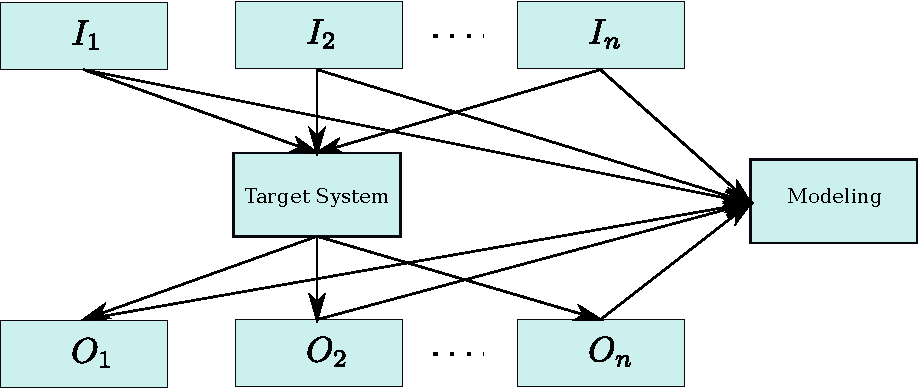
\includegraphics[width=2.5in]{system_identification_approach_offline.pdf}
  }\\
  \subfloat[ online]{
  	  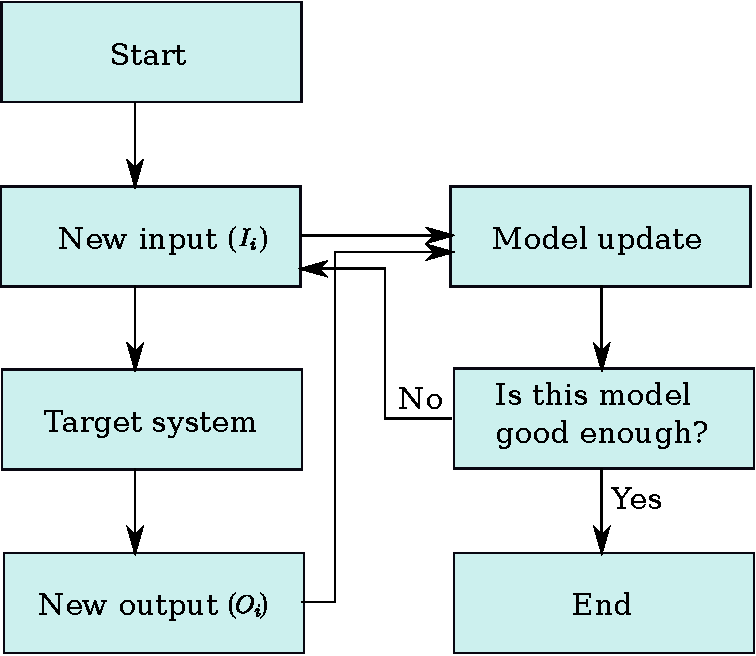
\includegraphics[width=2.5in]{system_identification_approach_online.pdf}
  }
  \caption{Diagrams showing two approaches for system identification. $(I_i, O_i)$, where $i \in \lbrace1, 2, \cdots, n\rbrace$, represent pairs of input and output data. Redrawn from \cite{Bongard_2005}}
  \label{fig:modeling_approaches}
\end{figure}

System identification can be divided into two main procedures: modeling and estimation. Modeling defines the order or general structure of the hidden system \cite{Fogel_1991}. Estimation identifies the parameters associated with the given structure. There are many algorithms to determine the parameters for a given structure. Typical estimation algorithms are recursive prediction error methods \cite{Ljungquist1993}, which are based on gradient search. Gradient search methods, such as greedy algorithm, may easily get trapped in local optima, especially when there are numerous local optima near the global optimum. An alternative search method is using evolutionary algorithms. There are some system identification methods that combine the modeling and estimation process, for example, the NARMAX method~\cite{Billings2013}. Neural networks can be also used, as their structure and weights (parameters) can be optimized simultaneously. The disadvantage of neural networks for modeling is they are difficult to interpret especially when consisting of multiple layers. Genetic programming provides an alternative way for finding the structure and parameters of the system. The models represented by genetic programming can be described in a tree-based structure. As the structure in genetic programming is evolving, the obtained model may be of a different structure in different runs~\cite{Vladislavleva:2009}. Bloating \cite{Eiben2003} is a problem in genetic programming, where the growth of the tree increases the complexity of the model structure. 
%As evolutionary algorithms use population-based search methods, this makes it more likely to get rid of local optima. 

Coevolutionary algorithms provide an effective way for system identification~\cite{Bongard2005}, \cite{Bongard_remote_robot_2004,Bongard_function_recovery_2004,Koos2009,Bongard2007PNAS,Mirm2011,Ly2014}. A range of work has been performed on simulated agents. In~\cite{Bongard_remote_robot_2004}, Bongard and Lipson proposed the \emph{estimation-exploration algorithm}, a nonlinear system identification method to coevolve inputs and models in a way that minimizes the number of inputs to be tested on the system. In each generation, the input that leads to the highest disagreement between the models' predicted output in simulation was carried out on the real system. The quality of the models was evaluated through quantitatively comparing the output of the real system and the models' prediction. The method was applied to evolve morphological parameters of a simulated quadrupedal robot after it undergoes `physical' damage. In a later work~\cite{Bongard_function_recovery_2004}, they reported that ``in many cases the simulated robot would exhibit wildly different behaviors even when it very closely approximated the damaged `physical' robot. This result is not surprising due to the fact that the robot is a highly coupled, non-linear system; thus similar initial conditions [...] are expected to rapidly diverge in behavior over time''. They addressed this problem by using a more refined comparison metric reported in~\cite{Bongard_function_recovery_2004}. In~\cite{Koos2009}, an algorithm which is also based on coevolution of models and inputs was presented to model the simulated quadrotor helicopter and improve the control quality. The inputs were selected based on multiobjective performances (e.g., disagreement ability of models as in ~\cite{Bongard_remote_robot_2004} and control quality of a given task). Models were then refined through comparing their prediction to each selected test trajectory. In~\cite{Kouchmeshky_2007}, the damage detection process is conducted by a coevolutionary algorithm to extract the maximum information from the system. In \cite{Mirmomeni_2011}, a coevolutionary algorithm is applied to estimate chaotic time series, in which the test data that can extract hidden information from the chaotic system co-evolves with the models. As in other system identification methods, predefined metrics play a critical role for evaluating the performance of models. 
  
Many studies also investigated the implementation of evolution directly in physical environments, on either a single robot~\cite{ Bongard-etal2006:science, Koos2013, Cully2015} or multiple robots~\cite{Alan2014}. In~\cite{Bongard-etal2006:science}, a four-legged robot was built to study how it can infer its own morphology through a process of continuous self-modeling. The robot ran a coevolutionary algorithm on-board. One population evolved models for the robot's morphology, while the other evolved actions (inputs) to be conducted on the robot for gauging the quality of these models through comparing sensor data collected. In~\cite{Alan2014}, a distributed coevolutionary approach was presented to coevolve on-board simulators and controllers of a group of ten robots to perform foraging behavior. Each robot has its own simulator which models the environment. The evolution of each robot's simulator was driven by comparing the real-world foraging efficiency (a pre-defined fitness metric) of its nearby neighbors each executing the best controller generated by their own simulators. Each robot has a population of controllers, which evolved according to the robot's on-board simulator. The best controller was chosen for performing real-world foraging. In all of the above approaches, the model optimization is based on pre-defined metrics (explicit or implicit), which are task dependent.

% This physical/embodied evolution helps reduce the \textit{reality gap} between the simulated and physical environments~\cite{Jakobi95}. 
%In \cite{Kouchmeshky_2007}, the damage detection process is conducted by coevolutionary algorithm to extract the maximum information from the system. In \cite{Mirmomeni_2011}, coevolutionary algorithm is applied to estimate chaotic time series, in which the test data that can extract information from the chaotic system co-evolves with the models. The approach described in~\cite{SchmidtLipson2009:science}, where the authors infer physical laws from observing mechanical systems, would also be applicable to learn about the behavior of an animal. Different from this approach our system learns about the behavior not through passive observation, but rather through an interactive process.

\section{Combining AI/Robotics and Animal Behavior}\label{sec:combine_AI_robotics_animal_behavior}

The variety of animal behaviors in nature is immense, ranging from simple perception of light to complicated behaviors such as navigation and communication. The scientific study of animal behavior is pursued not only because it is a subject of interest in itself, but also because the knowledge gained from it has several practical applications. In AI/Robotics, there is a large interest of studying animal behavior, as the model/knowledge learned can be used to build a more intelligent machine. At the same time, building a machine that mimics the animal helps researchers to better understand its behavior. In this section, we review how AI/robotics and animal behavior study benefit each other. 

This section is organized as follows. Section~\ref{sec:animal_behavior_in_nature} introduces a variety of animal behaviors observed in nature. Section~\ref{sec:swarm_optimization_swarm_robotics} details how animal behavior can be used as inspiration to solve engineering tasks, especially in the area of AI/robotics. Section~\ref{sec:contribution_of_AI/robotics_to_ethology} shows how AI/Robotics can contribute to ethology, which is the (ultimate) aim of this thesis.

\subsection{Animal Behavior in Nature}\label{sec:animal_behavior_in_nature}

Compared with the behaviors exhibited by complex animals such as mammals, insect behavior has been also widely studied by researchers. The simple neural system of insects makes it more feasible to replicate the intelligence. 

%(which is widely observed in animals such as insect larvae and worms~\citep{Fraenkel:DP:1961, Stephen:Op:1990})

A basic insect behavior is taxis, which is its intrinsic behavioral response to a specific stimulus. Taxis is divided into different types according to the stimulus. These behaviors include phototaxis (light), chemotaxis (chemicals), thermotaxis (temperature), etc. An interesting taxis behavior of crickets is that the female crickets perform complex auditory orientation behavior towards the male crickets. Researchers have found this complex sound localization behavior emerges from simple reactive steering responses to specific sound pulses generated by male crickets~\cite{Hedwig2004}. Apart from taxis behaviors, some insects use the stimuli as cues for navigation or migration. For instance, the bee uses its vision system to navigate in the air and avoid obstacles. Another interesting behavior found in insects is the ball movement of dung beetles~\cite{Emily_2012}. Once the dung beetles form the pieces of dung into a ball, they always roll the dung-ball in a straight line using various stimuli (e.g., the moon, sun and polarised light \cite{Byrne_2003, Matthews_1962}) as visual cues to transport the food source. This behavior ensures that they keep away from the competitors as far as possible. The stimulus-response behaviors in insects mentioned above are investigated by biologists for centuries. Although the behavior exhibited by insects may be simple and easy to mimic, it is not trivial to be modeled and well understood \cite{Ignacio2009}. When investigating such behaviors, biologists need to learn how to interact with the animal in a meaningful way to extract all of its behavioral repertoire. 
%However, whether this interacting ability could be exhibited by an intelligent machine is still an uncertain problem, which is addressed in this thesis. \textcolor{red}{For example, a lobster follows the salt-water plume---a kind of chemical signal to find the source.} 

Apart from the behavior of a single animal, swarm behaviors, which are emergent (collective) behaviors that arise from the interactions of a number of animals (especially social insects) in a group, have also been widely observed in nature. The individual behaviors in a swarm tend to be relatively simple~\cite{Camazine2001}. The global behavior that is exhibited in a swarm is a result of a self-organized process. Researchers found that individuals do not need the representation or complex knowledge to build a map of what the global behavior should be~\cite{Garnier:SI:2007}. From the point of control, swarm behavior is a distributed control system which does not rely on central coordination.

Many swarm behaviors are observed in nature. For example, the birds' flocking behavior is of particular interest to humans. This is not only because of their aesthetic shape formed in a group, but also because of the way the birds coordinate each other to maintain that shape. A simple mathematical model was proposed by~\cite{Craig:CG:1987} to describe the individual behavior of each bird in a flock. The three rules are: attraction, repulsion and alignment. In the attraction rule, the birds will be attracted by their neighbors, and this would result in each bird moving towards to the `center' of their neighbors. Repulsion means the bird needs to avoid colliding with each other. Alignment assumes that each bird moves in the same direction with its neighbors. Although there is no proof that flocking birds follow exactly the three rules, it is attractive that the boids (in simulation) following such simple rules can mimic the real flocking behavior closely. There are many other swarm behaviors which are also studied extensively such as the aggregation of cockroaches~\cite{Jeanson:AB:2005}, foraging in ants~\cite{Carroll1973}, flashing synchronization in fireflies~\cite{James:ARE:1971}, mound building in termites~\cite{Bruinsma:PHD:1979}. 

\subsection{Swarm Optimization and Swarm Robotics}\label{sec:swarm_optimization_swarm_robotics}

In this section, we review some techniques that are inspired by observation of animal behaviors. Section \ref{sec:swarm_optimization_related_work} reviews two bio-inspired algorithms---ant colony optimization algorithm~\cite{Dorigo_1997} and particle swarm optimization algorithm~\cite{Kennedy:ICNN:1995}. Section \ref{sec:swarm_robotics_related_work} introduces how the intelligence observed in animals can be applied in the field of robotics, in particular, swarm robotics.
%Swarm robotics which uses the swarm behavioral rules of social insects as an design principle to solve complex tasks has been paid much attention in recent decades. 

\subsubsection{Swarm Optimization}\label{sec:swarm_optimization_related_work}

\textbf{Ant Colony Optimization}

Ant Colony Optimization (ACO) was inspired by the foraging behavior of ants \cite{dorigo2008ant}. When an ant finds an item of food, it will leave pheromone on its path back to the nest. Other ants will be attracted by the pheromone, the strength of which may represent the quantity/quality of the food. Researchers have found that this indirect communication, which is know as \textit{stigmergy}~\cite{Holland:AL:1999}, leads them to find the shortest path between their nest and location of food source. The initial application of ACO is to find the optimal path in a combinational (discrete) problem. Note that nowadays the application of ACO algorithms ranges from discrete optimization (e.g., routing and load balancing~\cite{DiCaro:JAIR:1998}) to continuous optimization~\cite{Dorigo:LNCS:2004}.   

The principle of ACO algorithms can be summarized by the two steps as follows:

\begin{itemize}
\item Use the pheromone model (and heuristic model) to generate candidate solutions. The pheromone model is a parameterized probability distribution in the search space. The heuristic model could be the length of the segment chosen.

\item The candidate solutions are used as a bias for sampling high-quality solutions in the next iteration.
\end{itemize}

For a complete implementation of ACO algorithms, see \cite{dorigo2008ant}. 


\textbf{Particle Swarm Optimization}

Particle Swarm Optimization (PSO) is another optimization algorithm which is inspired by the flocking of birds and schooling of fish. It was first proposed by Kennedy and Eberhart~\cite{Kennedy:ICNN:1995}. The initial application is to optimize the weights of neural networks---a continuous optimization problem. It is also widely used in discrete optimization. 

The basic component in PSO is called \textit{particle}. A PSO algorithm consists of a finite set of particles. The movement of each particle is updated using \textit{velocity}. The velocity of each particle in each time step is updated based on its current velocity, the deviation between the best position (the particle has found so far) and its current position, and the deviation between the best position by its neighbors and its current position. This usually results in the particles moving towards the high-quality solutions after certain iterations. The update of each particle can be written using two equations as follows~\cite{Kennedy:ICNN:1995}:
\begin{equation}\label{eq:particle_velocity_update}
\overrightarrow{v}_{i+1} =  \overrightarrow{v_{i}} + c_1\overrightarrow{R_{1}}\otimes(\overrightarrow{p_{i}} - \overrightarrow{x_{i}}) + c_2\overrightarrow{R_{2}}\otimes(\overrightarrow{p_{g}} - \overrightarrow{x_{i}}). 
\end{equation} 

\begin{equation}\label{eq:particle_position_update}
\overrightarrow{x}_{i+1} =  \overrightarrow{x_{i}} + \overrightarrow{v_{i}}.
\end{equation} 

$\overrightarrow{R_{1}}$ and $\overrightarrow{R_{2}}$ are independent random number generators that return a vector of random values in range $[0, 1]$. $c_1$ and $c_2$ are referred to as acceleration coefficients. 
($\overrightarrow{p_{i}} - \overrightarrow{x_{i}}$) and ($\overrightarrow{p_{g}} - \overrightarrow{x_{i}}$) represent respectively the deviation between the best position (it has found so far) and its current position,  and deviation between the best position by its neighbors and its current position. The first item in Eq.~\eqref{eq:particle_velocity_update} keeps the particle moving in the previous direction; the second item makes the particle move towards the best position of its own; the third position forces the particle move towards to the best position that its neighbors have found. Eq.~\eqref{eq:particle_position_update} updates the particle's position.  
 
\subsubsection{Swarm Robotics}\label{sec:swarm_robotics_related_work}

In the previous section, we described how swarm behaviors have inspired the design of novel optimization algorithms. In this section, we introduce how to apply swarm intelligence techniques to multi-robot research, which is referred to as swarm robotics. The behavior of many social insects (e.g, ants, termites, wraps and bees) has been used as inspirations in swarm robotics. 

%To accomplish the same task, using a single expensive robot with complex control structure may be feasible; however it may have low efficiency and prone to failure. 
Swarm robotics investigates how multiple robots each with limited ability communicate, coordinate, and self-organize to accomplish certain tasks. The advantages of swarm robotics are as follows: 

\begin{itemize}

\item \textit{Robustness:}  The robustness of a swarm robotic system can be explained in the following: 1) A failure of a single robot does not influence other robots in the group; 2) the control is distributed; 3) as the individual is simple, it has fewer components that could fail. Note that swarm robotic systems can also be affected by errors. That is, some individuals' failure would influence the whole self-organized process~\cite{Bjerknes2013}.
%4) the perception from multiple robots would increase the system's robustness. 

\item \textit{Scalability:} In swarm robotics, a small change of the number of robots does not have significant impact on the global performance/behavior of the system (unless the number is sufficiently small). When investigating the performance of a swarm robotic system, a scalability study is usually considered~\cite{Jianing:TRO:2015, Melvin_DARS2014}.
%That is, increasing/decreasing the number of robots, the system should be still under control and the coordination is still maintained.

\item \textit{Flexibility:} The swarm could adapt to changing tasks and generate relevant solutions, by changing the role of each robot \cite{Sahin:LNCS:2005}. 
\end{itemize}

In order to coordinate, robots need to interact with each other and their environment. There are three kinds of interaction in swarm robotic systems \cite{Rodeirch2015}. 

\begin{itemize}

\item \textit{Interaction via environment:} Robots communicate by changing the environment. There is no explicit communication between each robot. In nature, the pheromone ants leave when foraging is an environmental stimulus for locating the food source.  

\item \textit{Interaction via perception:} Robots can perceive each other in a limited range. This perception is local and there is no explicit communication between the robots. The robots can distinguish different items (e.g., other robots, objects) in the environment. In nature, when ants need to collectively pull food to the nest, they need to perceive each other (to avoid collision) and the food (object).

\item \textit{Interaction via explicit communication:} This type of communication could be realized by broadcast (e.g., WiFi~\cite{Gerkey:TRA:2002}) or a distributed sensing network~\cite{Winfield:LNCS:2000}. How to build a reliable network when the number of robots is significantly large is still a topic widely discussed. When the number of robots increases, the load of communication increases exponentially. A possible solution is combining the advantage of network communication and local communication using the robots' perception.
%In this method, an instructure is required to communicate with a swarm of robots in real time. 

\end{itemize}

A range of tasks have been demonstrated in swarm robotics. The tasks range from aggregation~\cite{Trianni:LNCS:2003, Gauci2014_ijrr, Garnier:AL:2008, Jeanson:AB:2005}, dispersion~\cite{howard2002mobile, mclurkin2004distributed}, pattern formation~\cite{Fujibayashi:DARS:2002, Chen:AAMAS:2012}, collective movement~\cite{Turgut:SI:2008} to cooperative transport~\cite{Kube:AB:1993, Kube:RAS:2000,Gross:IJBC:2009, Jianing:TRO:2015}, etc. Aggregation can be considered as the fundamental behavior of other more complex tasks. In~\cite{Jeanson:AB:2005}, a group of robots mimic the cockroaches' aggregation behaviors, in which the robots join or leave a nest (place) in the environment with a probability proportional to the size of the nest. In~\cite{Gauci2014_ijrr}, the robots each with a binary sensor were reported to aggregate into a single cluster, validated using $40$ e-puck robots. The robots do not perform algorithmic computation. The aggregation performance scales well with $1000$ robots in simulation. In~\cite{Werfel:Sci:2014}, Werfel et al. designed a group of termite-inspired robots that work collectively to build several structures. The robots communicate with each other using \textit{stigmergy}. In~\cite{Turgut:SI:2008}, a group of nine Kobot robots were reported to mimic the flocking behavior of birds. These robots followed some simple rules similar to those proposed by Reynolds~\cite{Craig:CG:1987}. In cooperative transport, Chen et al.~\cite{Jianing:TRO:2015} presented a strategy for a group of miniature robots to transport a tall object to the goal. In the task, the robots only push the object when the robots' vision of the goal is occluded by the object. This strategy was proved to be able to push any convex object to the goal in a 2D environment. 
%The advantage of using stochastic algorithm is that they do not need to form a connected network in the initial configuration. 
\subsection{Contribution of AI/Robotics to Ethology}\label{sec:contribution_of_AI/robotics_to_ethology}

In the previous sections, it was reviewed how the study of animal behavior can be used as inspiration for designing optimization algorithms and robotic systems. However, AI/robotics can also benefit the study of animal behavior. This section reviews two approaches: \textit{learning from synthesis} and \textit{robot-animal interaction}.

\subsubsection{Learning from Synthesis}

Ethologists have studied animal behavior over a century. There are some basic steps that ethologists follow in the study of animal behavior~\cite{camazine2003self}. The first step is observation, and after that they formulate some scientific questions on the observed behavior, and generate hypothesis to answer these questions. They then conduct related experiments on the animals and collect data. After analyzing the data, the conclusion will be made to support or reject their hypothesis.

Robotics or artificial life can be used as an alternative methodology to investigate and understand animal behavior. Robots can be used as physical models of animal behaviors for testing hypotheses~\citep{Barbara_2000, Meyer2008}. For example, taxis behavior has often been implemented on mobile robotic systems for investigating steering and navigation \cite{Ignacio2009}. In~\citep{Barbara_1995}, Webb used a robot to model the phonotaxis behavior of crickets~\citep{Popov:JCP:1997}. The robot can locate the position of a sound source and moves towards it under different conditions. There was good agreement between data collected from experiments with the robot and animals. Another taxis behavior---chemotaxis in which animals follow a specific chemical trail has been used as a model for robots to find odor source based on artificial neural networks \cite{Farah_2002} and even Braitenberg vehicles \cite{Lilienthal_2003}. Robots can be used as a validation for the models obtained from biologists and allow them to better understand the animal behavior from a synthetic point of view. Besides, roboticists can generate new hypotheses and test them using (simulated or physical) robots. In social behavior study, Balch et al.~\citep{Balch_2006} built executable models of the behaviors of ants and monkeys, which can be directly executed by multi-robot systems. The aim is to show how research into multi-robot systems can contribute to the study of collective animal behaviors. In \cite{Chappell_2010}, Chappell et al. argue that there are many ways in which biologists interested in natural intelligence can learn from AI and robotics, and they outline specific kinds of contributions that AI can make to biological study. They also give some suggestions on how AI and robotics researchers could collaborate with biologists to solve some cutting-edge problems in animal behavior.
% Besides robotics, there are some researchers arguing that artificial intelligence can also make significant contributions to biological study. 

As opposed to the works mentioned above, the method proposed in this thesis aims to synthesize models of agent (animal) behaviors automatically, rather than manually. This could help to spare scientists from having to perform numerous laborious experiments, allowing them instead to focus on using the generated models to produce new hypotheses. 

\subsubsection{Robot--Animal Interaction}\label{sec:robot_animal_interaction}

Besides pure robot-based or AI research, researchers also use robots to interact with real animals. They build and program robots (i.e., replicas) that can be inserted into the group of social animals~\cite{Faria2010, Halloy2013, J.Halloy2007, Thomas2013, Vaughan2000}. Robots can be created and systematically controlled in such a way that they are accepted as con- or hetero-specifics by the animals in the group~\cite{Krause2011}. In this case, one ``animal'' in a group is completely controlled and they can observe the behaviors of the mixed society \cite{J.Halloy_2007}. The behavior of the inserted robot can be controlled and the model can also be embedded into the robot for verification \cite{Krause_2011}. The behavior of robots can be programmed in such a way that its behavior is not influenced by other animals in the group, and they can be used as demonstrators or leaders in the experiments. Further more, it is simpler to test a hypothesis through controlled interaction in social behaviors. 

In~\cite{Faria2010}, a replica fish which resembled the appearance (i.e., visual morphology) of sticklebacks was created to investigate two types of interaction: recruitment and leadership. In~\citep{Kopman2013}, a robot-fish that can interact intelligently with live zebrafish to study their preference and locomotion behavior was designed. In~\cite{J.Halloy2007}, autonomous robots which executed a derived model were mixed into a group of cockroaches to modulate their decision-making of selecting shelter in the aggregation behavior. The robots behaved in a similar way to the cockroaches. Although the robots' appearance was different to that of the cockroaches, the robots released a specific odor that the cockroaches could detect and regard the robots as conspecifics. In \cite{Vaughan_1998, Vaughan2000}, Vaughan et al. have built a mobile robot that can interact with ducks in a circular arena and drive them to the safe place. In \cite{Gribovskiy_2010}, Gribovskiy et al. designed a robot which is capable of interacting with chicks to study how the behavior of chicks is influenced by the others in a group.  

Although robots which are well designed can be mixed with social animals, building such kind of robot is a time-consuming process. It is also expensive to some extent and requires the collaboration of researchers from different disciplines. In the aforementioned works, the models were manually derived and the robots were only used for model validation. This robot-animal interaction framework could be enhanced through the system identification method proposed in this dissertation, which autonomously infers the collective behavior. 

\clearpage 

%The research of animal behavior has lasted for centuries. There are some basic steps that ethologists follow in the study of animal behavior. The first step is observation, and after that they formulate some scientific questions on the observed behavior, and generate hypothesis to answer these questions. In order to verify the hypothesis, they actively conduct related experiments in the real animals and collect certain amount of data. After analyzing the data, the conclusion will be made to support or reject their hypothesis. Take the behavior of dung beetle for instance. An interesting feature observed by ethologists in the behavior of dung beetles is that they always roll the dung-ball in a straight line. This strategy guarantees that the beetles can roll the dung as far as possible in the shortest time, ensuring that they can escape from the competition or danger that may occur near the cite of dung \cite{Emily_2012}. Previous works show that the most significant cues which dung beetles use for navigation -- straight line movement are the moon, sun and polarised light \cite{Byrne_2003, Matthews_1962}. In \cite{Dacke_2004}, Dacke, et al. study how dung beetle \textit{Scarabaeus zambesianus} orientates due to the artificial polarization pattern instead of observing the behavior in the natural polarized light, since it is quite easy to control the angle when using artificial light source. To do the experiment, they put the dung beetle in a squared arena. When the beetle enters the central point, they switch the angle of the artificial light source from 0 degree to 90 degree to interact with the dung beetle. Then they observe the path taken by the rolling dung to see whether the angle of light source has influence on the beetle's orientation behavior. The light switching process is very time-consuming, and the researchers have to change the angle of light source for many times (90 times, if the angle increases one degree each time). However, if this process is finished by a machine, it could free the ethologists from a lot of repetitive tasks, since the machine can shift the angle of light source as a grid of numeric values and observe the orientation of dung beetle under each specific condition. A high-capacity machine could observe this behavior without human intervention, generating thousands of experimental data very quickly. 